\chapter{Impact of the Project}
\section{Introduction}
By the year 2000, around 100 million people had access to the internet. Back then, it was considered a strange hobby to get engaged socially online.\\
By that time, the social network MySpace began raising awareness and became a popular place to create a profile and start adding more people. One could say that MySpace set the first tracks, which later would inspire and give birth in 2005 to the well-known Facebook.\\
One year later, out of the same inspiration was Twitter created. Ever since that happened, the number of active users in Twitter has exponentially grown. This can be shown in~\Cref{fig:twitterchart}.\\
Social networks are definitely an important agent in our lives. Ever since the beginning of these platforms, the developers have been trying to improve and enhance the capabilities of the platforms in order to ensure the user an exceptional quality of the social network. To this purpose, the platforms become more intelligent and offer more features. That is the reason why studying sarcasm detection can be very interesting.\\
In this appendix, the social, environmental and ethical impact of this project will be analyzed.
\begin{figure}
    \centering
    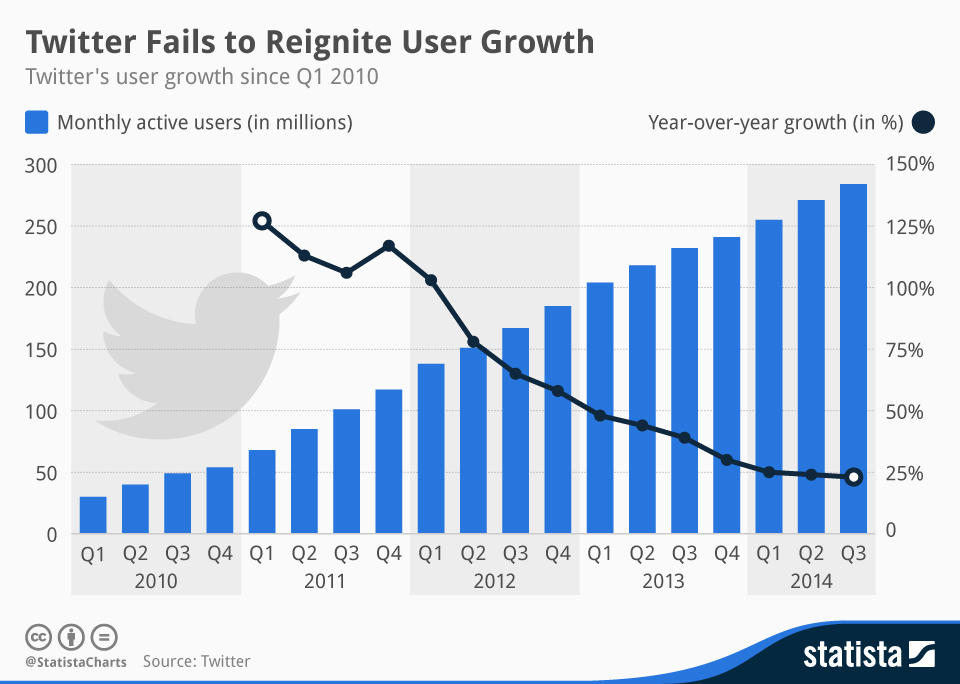
\includegraphics[scale=0.45]{img/twitter-chart.png}
    \caption{Twitter's popularity in the past years}
    \label{fig:twitterchart}
\end{figure}
\section{Social Impact}
There are two ways of uploading information into any social network: text and media content. This project will allow developers to detect sentiment in text. I believe that this project is a very powerful tool due to the ability to detect people's feelings towards a certain topic. To visualize the social impact of this project, an example will be given:\\
Let us imagine that the Spanish General Elections are taking place in three weeks from now. In such a period, political parties are focusing their efforts on attracting people. This is done through a political campaign. The idea behind it is to influence the decision-making process within a specific group. To do so, political leaders have always used the media and advertisements to present their ideas. If we think about this, there is no way of knowing precisely how good is a political leader performing before the elections day. In other words, how can a political leader now if the ideas presented are liked or disliked? Is it even possible to find a specific group where the ideas are liked?  Now, thanks to social networks the rules change because the citizen is allowed to react to the political ideas advertised by the political leader. Finally, the citizens have a way of individually tweet, like, dislike, retweet, etc.\\
In a big country, such as Spain with more than 46,000,000 citizens, one cannot go and read the reactions of millions of people. Even though social networks now allow the citizen to react to the political campaign, it is still very difficult for the political leader to understand precisely how do the people feel toward the ideas proposed.\\
This project brings an answer to that problem. By using the tools described in this project and setting adequate filters in Twitter, it is now possible to detect the sentiment of the citizens towards a political program. Furthermore, with the hashtag tool offered by Twitter, it is even easier to filter and analyze the desired tweets.\\
Companies are also very much interested in this project because now they have a way of analyzing how do people feel towards the product that the company offers. This project gives them the possibility of studying the market.\\
Finally, the privacy of the users is a very sensitive element in any data analysis project. This project data came from the Twitter database and it is open to the public.
\section{Environmental Impact}
This section will define the main environmental effects of this project.\\
Electronic equipment, such as computers, require a constant electric current flow to work. That current is manifested as a charge in the electricity network. If the organization uses efficient and class A computers, the energy consumption can be significantly reduced. However, there is no way of totally obliterating the energy demand.\\ Moreover, in case laptops were used, there would be an environmental threat due to the batteries. That is why laptops are not recommended.
\section{Ethical Impact}
One important ethical implication is the fact that automating activities implies job loss. If a program can predict the sentiment of the people with a reasonable level of accuracy, then there is no need to employ someone to do that task. However, the mere use of this project requires new jobs to maintain the system.\\
Secondly, a very serious and sensitive implication is the use of people's data. The privacy policy used by Twitter indicates that the user consents the use of the data stored in Twitter. 


